% GNUPLOT: LaTeX picture with Postscript
\begingroup
  \makeatletter
  \providecommand\color[2][]{%
    \GenericError{(gnuplot) \space\space\space\@spaces}{%
      Package color not loaded in conjunction with
      terminal option `colourtext'%
    }{See the gnuplot documentation for explanation.%
    }{Either use 'blacktext' in gnuplot or load the package
      color.sty in LaTeX.}%
    \renewcommand\color[2][]{}%
  }%
  \providecommand\includegraphics[2][]{%
    \GenericError{(gnuplot) \space\space\space\@spaces}{%
      Package graphicx or graphics not loaded%
    }{See the gnuplot documentation for explanation.%
    }{The gnuplot epslatex terminal needs graphicx.sty or graphics.sty.}%
    \renewcommand\includegraphics[2][]{}%
  }%
  \providecommand\rotatebox[2]{#2}%
  \@ifundefined{ifGPcolor}{%
    \newif\ifGPcolor
    \GPcolorfalse
  }{}%
  \@ifundefined{ifGPblacktext}{%
    \newif\ifGPblacktext
    \GPblacktexttrue
  }{}%
  % define a \g@addto@macro without @ in the name:
  \let\gplgaddtomacro\g@addto@macro
  % define empty templates for all commands taking text:
  \gdef\gplbacktext{}%
  \gdef\gplfronttext{}%
  \makeatother
  \ifGPblacktext
    % no textcolor at all
    \def\colorrgb#1{}%
    \def\colorgray#1{}%
  \else
    % gray or color?
    \ifGPcolor
      \def\colorrgb#1{\color[rgb]{#1}}%
      \def\colorgray#1{\color[gray]{#1}}%
      \expandafter\def\csname LTw\endcsname{\color{white}}%
      \expandafter\def\csname LTb\endcsname{\color{black}}%
      \expandafter\def\csname LTa\endcsname{\color{black}}%
      \expandafter\def\csname LT0\endcsname{\color[rgb]{1,0,0}}%
      \expandafter\def\csname LT1\endcsname{\color[rgb]{0,1,0}}%
      \expandafter\def\csname LT2\endcsname{\color[rgb]{0,0,1}}%
      \expandafter\def\csname LT3\endcsname{\color[rgb]{1,0,1}}%
      \expandafter\def\csname LT4\endcsname{\color[rgb]{0,1,1}}%
      \expandafter\def\csname LT5\endcsname{\color[rgb]{1,1,0}}%
      \expandafter\def\csname LT6\endcsname{\color[rgb]{0,0,0}}%
      \expandafter\def\csname LT7\endcsname{\color[rgb]{1,0.3,0}}%
      \expandafter\def\csname LT8\endcsname{\color[rgb]{0.5,0.5,0.5}}%
    \else
      % gray
      \def\colorrgb#1{\color{black}}%
      \def\colorgray#1{\color[gray]{#1}}%
      \expandafter\def\csname LTw\endcsname{\color{white}}%
      \expandafter\def\csname LTb\endcsname{\color{black}}%
      \expandafter\def\csname LTa\endcsname{\color{black}}%
      \expandafter\def\csname LT0\endcsname{\color{black}}%
      \expandafter\def\csname LT1\endcsname{\color{black}}%
      \expandafter\def\csname LT2\endcsname{\color{black}}%
      \expandafter\def\csname LT3\endcsname{\color{black}}%
      \expandafter\def\csname LT4\endcsname{\color{black}}%
      \expandafter\def\csname LT5\endcsname{\color{black}}%
      \expandafter\def\csname LT6\endcsname{\color{black}}%
      \expandafter\def\csname LT7\endcsname{\color{black}}%
      \expandafter\def\csname LT8\endcsname{\color{black}}%
    \fi
  \fi
  \setlength{\unitlength}{0.0500bp}%
  \begin{picture}(6000.00,4500.00)%
    \gplgaddtomacro\gplbacktext{%
      \csname LTb\endcsname%
      \put(946,704){\makebox(0,0)[r]{\strut{} 0}}%
      \put(946,1014){\makebox(0,0)[r]{\strut{} 0.2}}%
      \put(946,1325){\makebox(0,0)[r]{\strut{} 0.4}}%
      \put(946,1635){\makebox(0,0)[r]{\strut{} 0.6}}%
      \put(946,1946){\makebox(0,0)[r]{\strut{} 0.8}}%
      \put(946,2256){\makebox(0,0)[r]{\strut{} 1}}%
      \put(1078,484){\makebox(0,0){\strut{} 0}}%      
      \put(1609,484){\makebox(0,0){\strut{} 1}}%      
      \put(2141,484){\makebox(0,0){\strut{} 2}}%      
      \put(2672,484){\makebox(0,0){\strut{} 3}}%      
      \put(3203,484){\makebox(0,0){\strut{} 4}}%
      \put(376,1480){\rotatebox{-270}{\makebox(0,0){\strut{}ITPC}}}%
      \put(2140,154){\makebox(0,0){\strut{}frequency, Hz}}%
      \put(2141,2400){\makebox(0,0){\strut{} \bf{MP}}}%             


      \put(3946,704){\makebox(0,0)[r]{\strut{} 0}}%
      \put(3946,1014){\makebox(0,0)[r]{\strut{} 0.2}}%
      \put(3946,1325){\makebox(0,0)[r]{\strut{} 0.4}}%
      \put(3946,1635){\makebox(0,0)[r]{\strut{} 0.6}}%
      \put(3946,1946){\makebox(0,0)[r]{\strut{} 0.8}}%
      \put(3946,2256){\makebox(0,0)[r]{\strut{} 1}}%
      \put(4078,484){\makebox(0,0){\strut{} 0}}%      
      \put(4609,484){\makebox(0,0){\strut{} 1}}%      
      \put(5141,484){\makebox(0,0){\strut{} 2}}%      
      \put(5672,484){\makebox(0,0){\strut{} 3}}%      
      \put(6203,484){\makebox(0,0){\strut{} 4}}%
%      \put(3176,1480){\rotatebox{-270}{\makebox(0,0){\strut{}ITPC}}}%
      \put(5140,154){\makebox(0,0){\strut{}frequency, Hz}}%
      \put(5141,2400){\makebox(0,0){\strut{} \bf{random}}}%             

      \put(946,3004){\makebox(0,0)[r]{\strut{} 0}}%
      \put(946,3314){\makebox(0,0)[r]{\strut{} 0.2}}%
      \put(946,3625){\makebox(0,0)[r]{\strut{} 0.4}}%
      \put(946,3935){\makebox(0,0)[r]{\strut{} 0.6}}%
      \put(946,4246){\makebox(0,0)[r]{\strut{} 0.8}}%
      \put(946,4556){\makebox(0,0)[r]{\strut{} 1}}%
      \put(1078,2784){\makebox(0,0){\strut{} 0}}%
      \put(1609,2784){\makebox(0,0){\strut{} 1}}%      
      \put(2141,2784){\makebox(0,0){\strut{} 2}}%      
      \put(2672,2784){\makebox(0,0){\strut{} 3}}%      
      \put(3203,2784){\makebox(0,0){\strut{} 4}}%
      \put(376,3980){\rotatebox{-270}{\makebox(0,0){\strut{}ITPC}}}%
            \put(2141,4700){\makebox(0,0){\strut{} \bf{AN}}}%      
 %     \put(2140,2154){\makebox(0,0){\strut{}frequency, Hz}}%

      \put(3946,3004){\makebox(0,0)[r]{\strut{} 0}}%
      \put(3946,3314){\makebox(0,0)[r]{\strut{} 0.2}}%
      \put(3946,3625){\makebox(0,0)[r]{\strut{} 0.4}}%
      \put(3946,3935){\makebox(0,0)[r]{\strut{} 0.6}}%
      \put(3946,4246){\makebox(0,0)[r]{\strut{} 0.8}}%
      \put(3946,4556){\makebox(0,0)[r]{\strut{} 1}}%
      \put(4078,2784){\makebox(0,0){\strut{} 0}}%      
      \put(4609,2784){\makebox(0,0){\strut{} 1}}%      
      \put(5141,2784){\makebox(0,0){\strut{} 2}}%      
      \put(5672,2784){\makebox(0,0){\strut{} 3}}%      
      \put(6203,2784){\makebox(0,0){\strut{} 4}}%
                  \put(5141,4700){\makebox(0,0){\strut{} \bf{AV}}}%             
 %     \put(3176,4480){\rotatebox{-270}{\makebox(0,0){\strut{}ITPC}}}%
 %     \put(5140,2154){\makebox(0,0){\strut{}frequency, Hz}}%
}%
    \gplgaddtomacro\gplfronttext{%
    }%
    \gplbacktext
    \put(0,2300){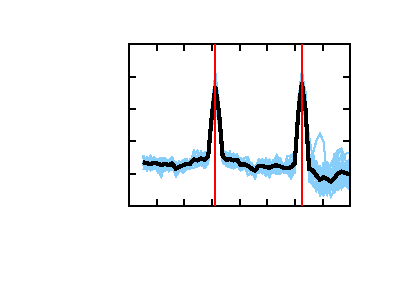
\includegraphics{./Figure_Simulated/anan_simulated}}%TL
    \put(3000,2300){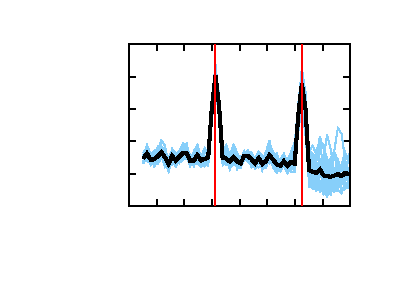
\includegraphics{./Figure_Simulated/avav_simulated}}%TR    
    \put(0,0){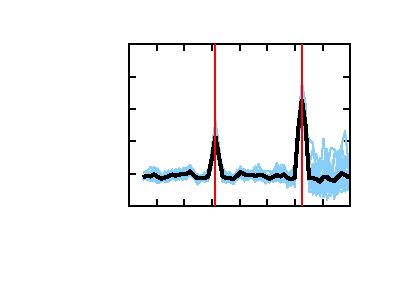
\includegraphics{./Figure_Simulated/phmi_simulated}}%BL
    \put(3000,0){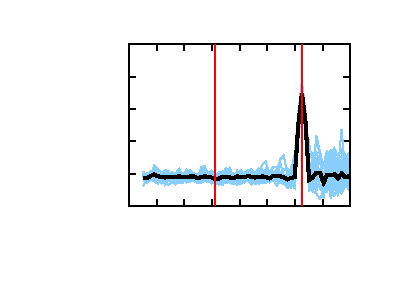
\includegraphics{./Figure_Simulated/rrrr_simulated}}%BR
    \gplfronttext
  \end{picture}%
\endgroup
